\documentclass[problems]{esg8012pset} 
  \usepackage{amsmath}
  \usepackage{amssymb}
  \usepackage{amsthm}
  \usepackage{enumerate}
  \usepackage{graphicx}
  \usepackage{hyperref}
  %\usepackage{siunitx}
  \providecommand{\uvec}[1]{{\hat{\bf{#1}}}}
  \usepackage{pgf,tikz}
  \usetikzlibrary{arrows}
  \usepackage{wasysym}
  \makeatletter
  \newcommand{\interitemtext}[1]{%
    \begin{list}{}
     {\itemindent=0mm\labelsep=0mm
     \labelwidth=0mm\leftmargin=0mm
     \addtolength{\leftmargin}{-\@totalleftmargin}}
      \item #1
    \end{list}
  }
  \makeatother
  \renewcommand{\d}{\,d}
  \providecommand{\norm}[1]{\lVert#1\rVert}
  \newtheorem{thm}{Theorem}[section]
  \newtheorem*{thm*}{Theorem}
\classname{Physics 8.012} 
\semester{Fall 2010} 
\problemsetnumber{9} 
\date{\today } 
\duedate{Monday, November 22} 
\readingassignment{Kleppner and Kolenkow, \emph {An Introduction to Mechanics}, Chapter Six} 
\begin{document}
\section{Problem \thesection: K\&K 6.14}
  A uniform stick of mass $m$ and length $l$ is suspended horizontally with end $B$ at the edge of a table and the other end $A$ is held by hand. Point A is suddenly released. At the instant after release:
  \begin{center}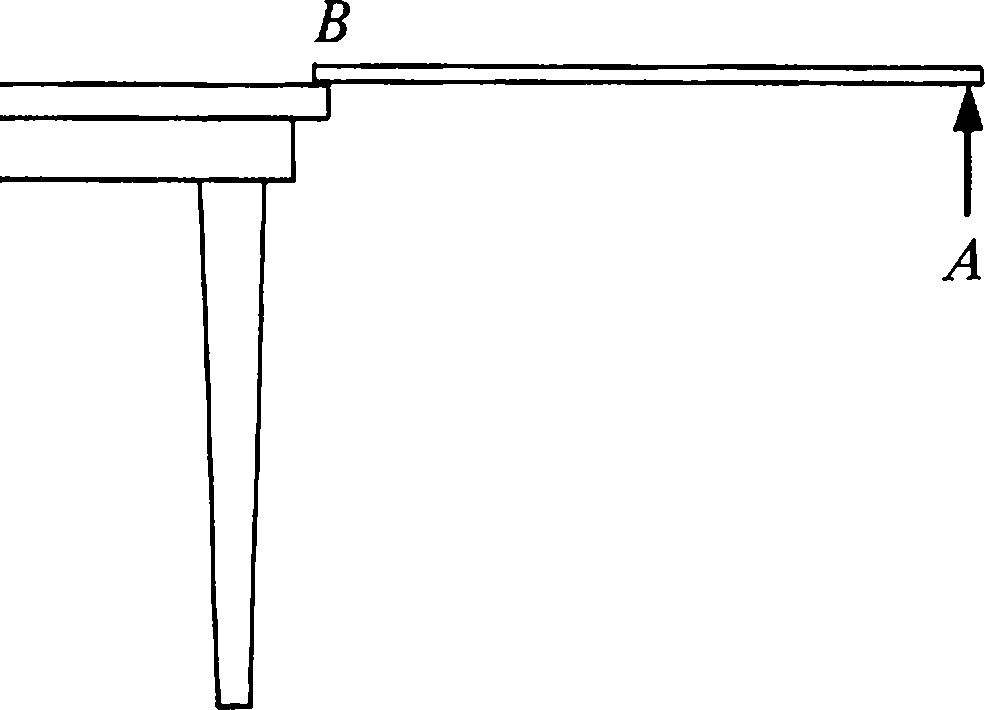
\includegraphics[width=0.33\textwidth]{ps09_1}\end{center}
  \begin{enumerate}[(a)]
    \item What is the torque about the end $B$ on the table?
    \item What is the angular acceleration about the end $B$ on the table?
    \item What is the vertical acceleration of the center of mass?
    \item What is the vertical component of the hinge force at $B$? Does the hinge force have a horizontal component at the instant after release?
  \end{enumerate}
\section{Problem \thesection: K\&K 6.18}
  A physical pendulum consists of a disc of radius $R$ and mass $m_d$ fixed at the end of a rod of mass $m_r$ and length $l$.
  \begin{center}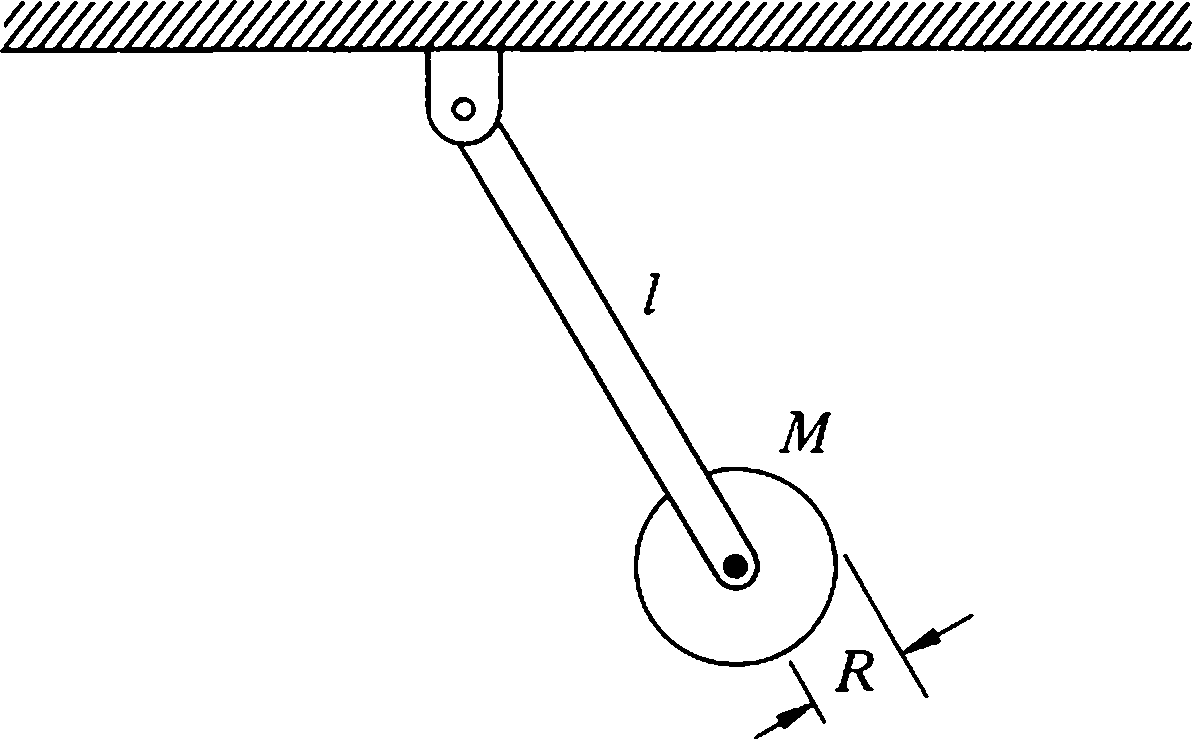
\includegraphics[width=0.3\textwidth]{ps09_2}\end{center}
  \begin{enumerate}[(a)]
    \item Find the period of the pendulum.
    \item How does the period change if the disk is mounted to the rod by a frictionless bearing so that it is perfectly free to spin?
  \end{enumerate}
\section{Problem \thesection: K\&K 6.24}
  A drum $A$ of mass $m$ and radius $R$ is suspended from a drum $B$ also of mass $m$ and radius $R$, which is free to rotate about its axis. The suspension is in the form of a massless metal tape wound around the outside of each drum, and free to unwind. Gravity is directed downwards. Both drums are initially at rest. Find the initial acceleration of drum $A$, assuming that it moves straight down.
  \begin{center}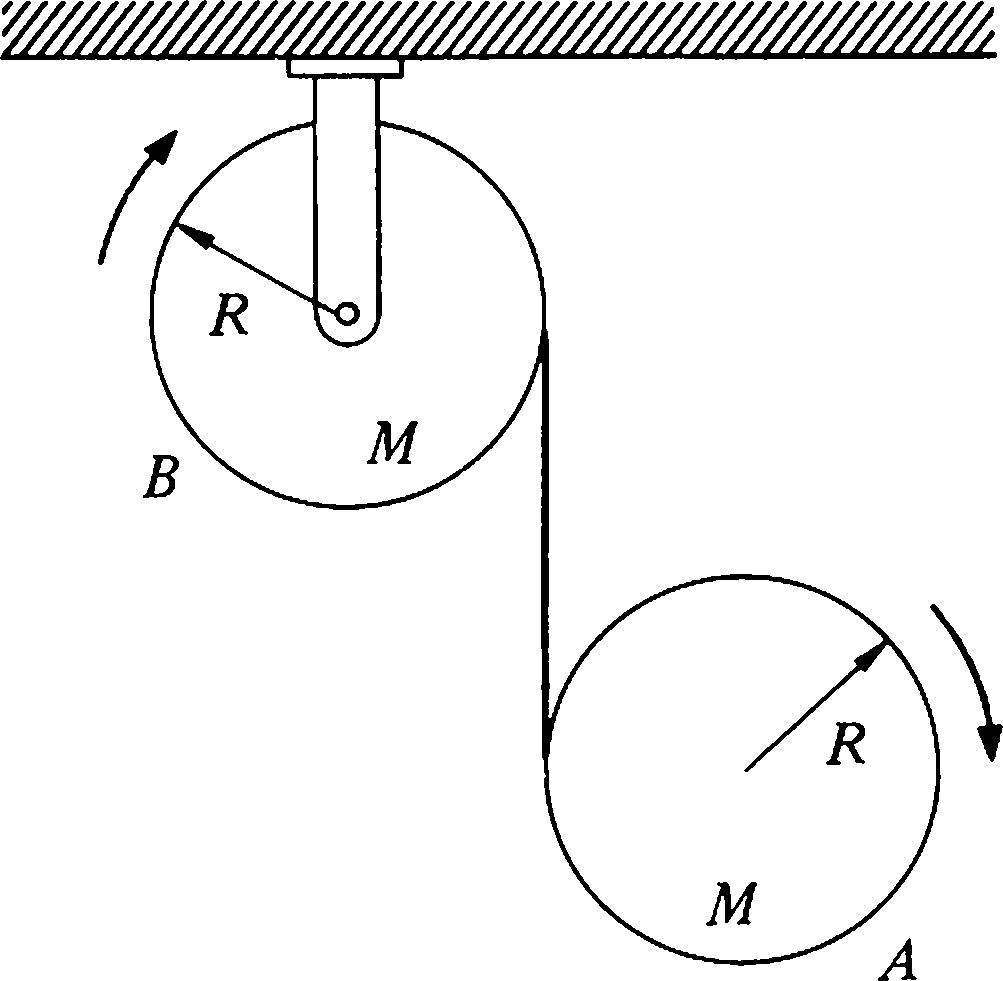
\includegraphics[width=0.25\textwidth]{ps09_3}\end{center}
\section{Problem \thesection: K\&K 6.29}
  A Yo-Yo of mass $m$ has an axle of radius $b$ and a spool of radius $R$. It's moment of inertia can be taken to be $I = (1/2)mR^2$ and the thickness of the string can be neglected.

  The Yo-Yo is released from rest.
  \begin{center}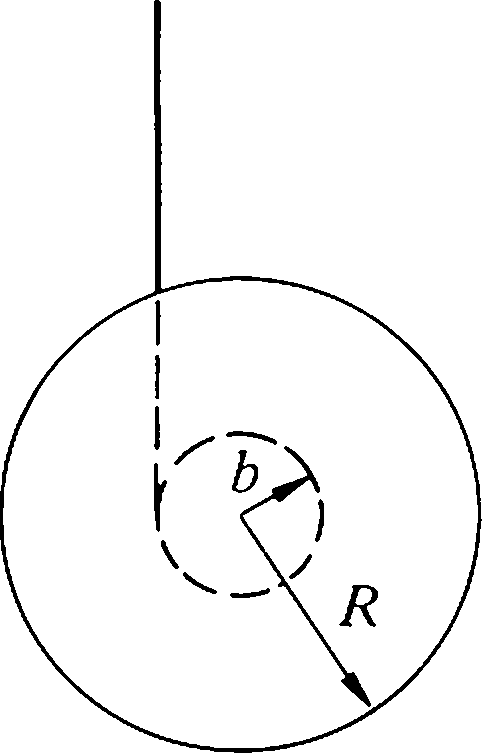
\includegraphics[width=0.15\textwidth]{ps09_4}\end{center}
  \begin{enumerate}[(a)]
    \item What is the tension in the cord as the Yo-Yo descends and as it ascends?
    \item The center of the Yo-Yo descends a distance $h$ before the string is fully unwound. Use conservation of energy to find the angular velocity of the Yo-Yo when it reaches its lowest point.
    \item What happens to the Yo-Yo at the bottom of the string?
    \item Assuming it reverses direction with uniform angular velocity, find the average force on the string while the Yo-Yo turns around.
  \end{enumerate}
\section{Problem \thesection: K\&K 6.30}
  A bowling ball of mass $m$ and radius $R$ is initially thrown down an alley with an initial velocity $v_0$ and it slides without rolling but due to friction it begins to roll. The moment of inertia of the ball about its center of mass is $I_\text{cm} = (2/5) mR^2$. What is the velocity of the bowling ball when its just start to roll without slipping.
  \begin{center}
    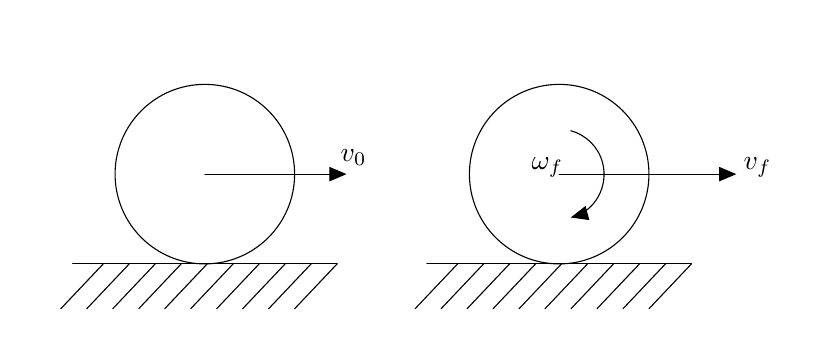
\begin{tikzpicture}[line cap=round,line join=round,>=triangle 45,x=3.0cm,y=3.0cm]
    \clip(-1.5,-0.25) rectangle (1.75,1);
    \draw(0.75,0.38) circle (0.38);
    \draw(-0.75,0.38) circle (0.38);
    \draw [->] (-0.75,0.38) -- (-0.15,0.38);
    \draw [->] (0.75,0.38) -- (1.5,0.38);
    %\draw [shift={(-0.75,0.38)},->] (-75:0.19) arc (75:0.19);
    %\draw [shift={(-0.75,0.38)},color=black,<-] (-75:0.19) arc (-75:75:0.19);
    \draw [shift={(0.75,0.38)},color=black,<-] (-75:0.19) arc (-75:75:0.19);
    %\draw [shift={(-0.75,0.38)}] plot[domain=-1.18:1.18,variable=\t]({1*0.19*cos(\t r)+0*0.19*sin(\t r)},{0*0.19*cos(\t r)+1*0.19*sin(\t r)});
    %\draw [shift={(0.75,0.38)}] plot[domain=-1.18:1.18,variable=\t]({1*0.19*cos(\t r)+0*0.19*sin(\t r)},{0*0.19*cos(\t r)+1*0.19*sin(\t r)});
    \draw (-1.31,0)-- (-0.19,0);
    \draw (0.19,0)-- (1.31,0);
    \draw (-0.19,0)-- (-0.37,-0.19);
    \draw (1.31,0)-- (1.13,-0.19);
    \draw (-0.3,0)-- (-0.48,-0.19);
    \draw (-0.41,0)-- (-0.59,-0.19);
    \draw (-0.52,0)-- (-0.7,-0.19);
    \draw (-0.63,0)-- (-0.81,-0.19);
    \draw (-0.74,0)-- (-0.92,-0.19);
    \draw (-0.85,0)-- (-1.03,-0.19);
    \draw (-0.96,0)-- (-1.14,-0.19);
    \draw (-1.07,0)-- (-1.25,-0.19);
    \draw (-1.18,0)-- (-1.36,-0.19);
    \draw (1.2,0)-- (1.02,-0.19);
    \draw (1.09,0)-- (0.91,-0.19);
    \draw (0.98,0)-- (0.8,-0.19);
    \draw (0.87,0)-- (0.69,-0.19);
    \draw (0.76,0)-- (0.58,-0.19);
    \draw (0.65,0)-- (0.47,-0.19);
    \draw (0.54,0)-- (0.36,-0.19);
    \draw (0.43,0)-- (0.25,-0.19);
    \draw (0.32,0)-- (0.14,-0.19);
    \draw[color=black] (-0.12,0.45) node {$v_0$};
    \draw[color=black] (1.59,0.41) node {$v_f$};
    %\draw[color=black] (-0.85,0.41) node {$\omega_0$};
    \draw[color=black] (0.7,0.41) node {$\omega_f$};
    \end{tikzpicture}
  \end{center}
\section{Problem \thesection: K\&K 6.37}
  A hockey puck of mass $m_1$ slides along ice with a velocity $v_0$ and strikes one end of a stick lying on the ice of length $l_2$ and mass $m_2$. The center of mass of the stick moves with an unknown magnitude $v_{cm}$. The stick also rotates about the center of mass with unknown angular velocity $\omega_{f}$. The puck continues to move in the same straight line as before it hit the stick with velocity $v_f$. Assume the ice is frictionless and there is no loss of mechanical energy during the collision.
  \begin{center}
    \begin{tikzpicture}[line cap=round,line join=round,>=triangle 45,x=2.0cm,y=2.0cm]
    \clip(-2,-1.5) rectangle (2.5,1.75);
    \draw [shift={(1.4,0)},->] (-75:0.5) arc (-75:75:0.5);
    \draw [->] (0,0.33) -- (0,1);
    \draw [->] (0,-0.33) -- (0,-1);
    \draw (-0.1,0.19) node[anchor=north west] {$\ell_2$};
    \draw (-1.1,1)-- (-0.9,1);
    \draw (-0.9,1)-- (-0.9,-1);
    \draw (-0.9,-1)-- (-1.1,-1);
    \draw (-1.1,-1)-- (-1.1,1);
    \draw (0.9,1)-- (1.1,1);
    \draw (1.1,1)-- (1.1,-1);
    \draw (1.1,-1)-- (0.9,-1);
    \draw (0.9,-1)-- (0.9,1);
    \draw(-1.77,-1) circle (0.1cm);
    \draw(1.77,-1) circle (0.1cm);
    \draw [->] (-1.65,-1) -- (-1.35,-1);
    \draw [->] (1.89,-1) -- (2.19,-1);
    \draw [->] (1,0) -- (1.4,0);
    \draw (-1.1,0.17) node[anchor=north west] {$x$};
    \draw[color=black] (-1.76,-1.15) node {$m_1$};
    \draw[color=black] (1.79,-1.17) node {$m_1$};
    \draw[color=black] (-1.25,-1) node {$v_0$};
    \draw[color=black] (2.3,-1) node {$v_f$};
    \draw[color=black] (1.63,0) node {$v_\text{cm}$};
    \draw[color=black] (2.09,0) node {$\omega_f$};
    \draw (-1.5,1.05) node[anchor=north west] {$m_{2}$};
    \end{tikzpicture}
  \end{center}
  \begin{enumerate}[(a)]
    \item Write down the equation for conservation of momentum.
    \item Write down the equation for conservation of energy.
    \item Is there any external torques acting on the system consisting of the puck and the stick? Write down the equation for conservation of angular momentum about a convenient point.
    \item Find the velocity of the center of mass of the stick.
    \item Find the velocity of the puck after the collision.
    \item Find the angular velocity of the stick after the collision.
  \end{enumerate}
\section{Problem \thesection: K\&K 6.41}
  A plank of length $2 l$ leans against a wall. The mass of the plank is m which is uniformly distributed. The plank is initially inclined at an angle $\theta$ with respect to the horizontal. It starts to slip downward without friction.
  \begin{center}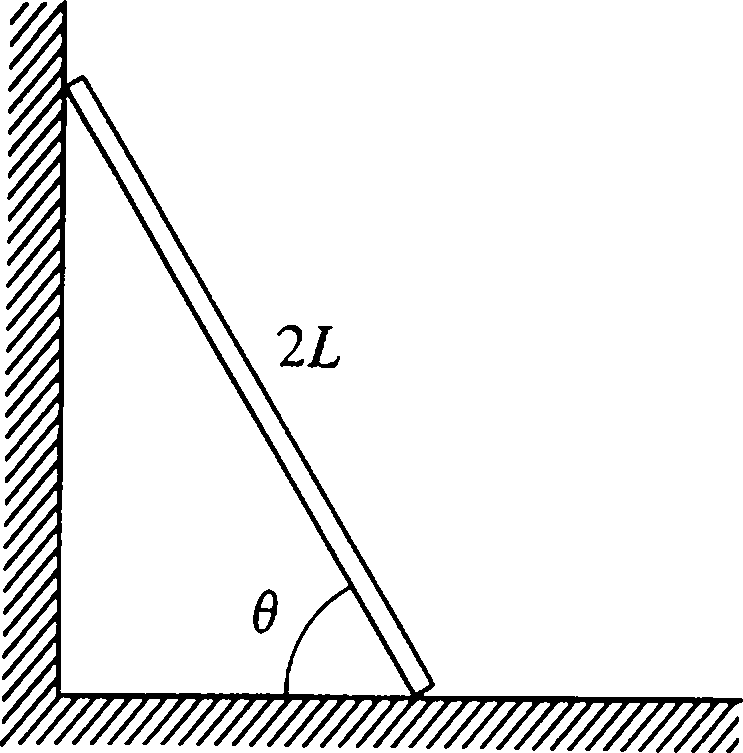
\includegraphics[width=0.25\textwidth]{ps09_7}\end{center}
  \begin{enumerate}[(a)]
    \item Draw a force diagrams showing all the forces acting on the plank. What is the condition that the plank just starts to slip from the wall.
    \item Is the mechanical energy of the plank conserved as it slips down the wall?
    \item What equations arise from the conditions for static equilibrium for both forces and torque? Think about which point to compute the torque about.
    \item Show that the top of the plank loses contact with the wall when it is two-thirds of its initial height against the wall. Hint: only a single variable and its derivatives are needed to describe the motion of the system. Consider the motion of the center of mass of the plank.
  \end{enumerate}
\end{document}
